\documentclass[a4paper]{article}
\usepackage[utf8]{inputenc}
\usepackage[margin=0pt]{geometry}
\usepackage{tikz}
\usetikzlibrary{shapes.misc}
\usepackage{xcolor}
\definecolor{discordblack}{HTML}{0f0f0f}
\usepackage{graphicx}
\usepackage{lmodern} % Adds scalable fonts to support large sizes
\usepackage[hidelinks]{hyperref}

\newcommand{\chip}[1]{%
    \tikz[baseline]
    \node[anchor=base, draw=none, fill=white, rounded rectangle, inner ysep=3.5pt, inner xsep=7pt, text height=1.5ex, text depth=0.5ex, text=discordblack, font=\small\sffamily\bfseries] {#1};%
}
\newcommand{\blackchip}[1]{%
    \tikz[baseline]
    \node[anchor=base, draw=none, fill=discordblack, rounded rectangle, inner ysep=3pt, inner xsep=7pt, text height=1.6ex, text depth=0.4ex, text=white, font=\normalsize\sffamily\bfseries] {#1};%
}
\newcommand{\blackchiphref}[2]{%
    \href{#1}{\tikz[baseline]\node[anchor=base, draw=none, fill=discordblack, rounded rectangle, inner ysep=3pt, inner xsep=7pt, text height=1.6ex, text depth=0.4ex, text=white, font=\normalsize\sffamily\bfseries] {#2};}%
}

% --- Lucide-style Icons using TikZ ---
\newcommand{\iconTerminal}{%
    \tikz[baseline=-0.7ex, line width=1.6pt, line cap=round, line join=round, scale=0.09]{
        \draw[white] (-3,-2) -- (-1,0) -- (-3,2);
        \draw[white] (0,-2) -- (3,-2);
    }%
}
\newcommand{\iconWeb}{%
    \tikz[baseline=-0.7ex, line width=1.6pt, line cap=round, line join=round, scale=0.09]{
        \draw[white] (0,0) circle (3);
        \draw[white] (-3,0) -- (3,0);
        \draw[white] (0,-3) -- (0,3);
        \draw[white] (0,0) ellipse (1.2 and 3);
    }%
}
\newcommand{\iconMobile}{%
    \tikz[baseline=-0.7ex, line width=1.6pt, line cap=round, line join=round, scale=0.09]{
        \draw[white, rounded corners=1pt] (-2,-3) rectangle (2,3);
        \draw[white] (-0.7,-2.2) -- (0.7,-2.2);
    }%
}
\newcommand{\iconLoop}{%
    \tikz[baseline=-0.7ex, line width=1.6pt, line cap=round, line join=round, scale=0.09]{
        \draw[white] (0,0) .. controls (2,1.8) and (3.5,1) .. (3.5,0)
                   .. controls (3.5,-1) and (2,-1.8) .. (0,0)
                   .. controls (-2,1.8) and (-3.5,1) .. (-3.5,0)
                   .. controls (-3.5,-1) and (-2,-1.8) .. (0,0);
    }%
}
\newcommand{\iconDB}{%
    \tikz[baseline=-0.7ex, line width=1.6pt, line cap=round, line join=round, scale=0.09]{
        \draw[white] (0,2) ellipse (3 and 1.2);
        \draw[white] (3,2) -- (3,-2);
        \draw[white] (-3,2) -- (-3,-2);
        \draw[white] (3,-2) arc (0:-180:3 and 1.2);
        \draw[white] (3,0) arc (0:-180:3 and 1.2);
    }%
}
\newcommand{\iconCube}{%
    \tikz[baseline=-0.7ex, line width=1.6pt, line cap=round, line join=round, scale=0.09]{
        \draw[white] (-3,1.5) -- (0,3) -- (3,1.5) -- (0,0) -- cycle;
        \draw[white] (-3,1.5) -- (-3,-1.5) -- (0,-3) -- (0,0);
        \draw[white] (3,1.5) -- (3,-1.5) -- (0,-3);
        \draw[white] (0,0) -- (0,-3);
    }%
}

% Dotted separator for sidebar skills (white)
\newcommand{\skillRow}[2]{%
    \noindent
    \begin{minipage}[t]{0.05\paperwidth}
        #1
    \end{minipage}%
    \hfill
    \begin{minipage}[t]{0.2\paperwidth}
        \raggedleft
        \linespread{1.3}\selectfont
        #2
    \end{minipage}
    \par
    \vspace{4pt}
    \noindent\tikz\draw[dotted, white, thick] (0,0) -- (\linewidth,0);
    \par
    \vspace{4pt}
}

% Consistent dotted separator for main content
\newcommand{\dottedSep}{%
    \par\vspace{5pt}%
    \noindent\tikz\draw[dotted, discordblack, thick] (0,0) -- (\linewidth,0);%
    \par\vspace{5pt}%
}

\begin{document}
\pagestyle{empty}

\begin{tikzpicture}[remember picture,overlay]
    % Black Sidebar (Left 1/3)
    \fill[discordblack] (current page.north west) rectangle ++(0.33333\paperwidth,-\paperheight);
    % Black Topbar (Top 1/3)
    \fill[discordblack] (current page.north west) rectangle ++(\paperwidth,-0.33333\paperwidth);

    % Rounding the inner corner (Intersection of white area)
    \fill[discordblack] ([xshift=0.33333\paperwidth, yshift=-0.33333\paperwidth]current page.north west)
        -- ++(1cm, 0)
        arc[start angle=90, end angle=180, radius=1cm]
        -- cycle;

    % Photo (Centered in the top-left square area)
    \node[circle, draw=white, ultra thick, minimum size=5cm, inner sep=0pt, path picture={
        \node at (path picture bounding box.center) {
            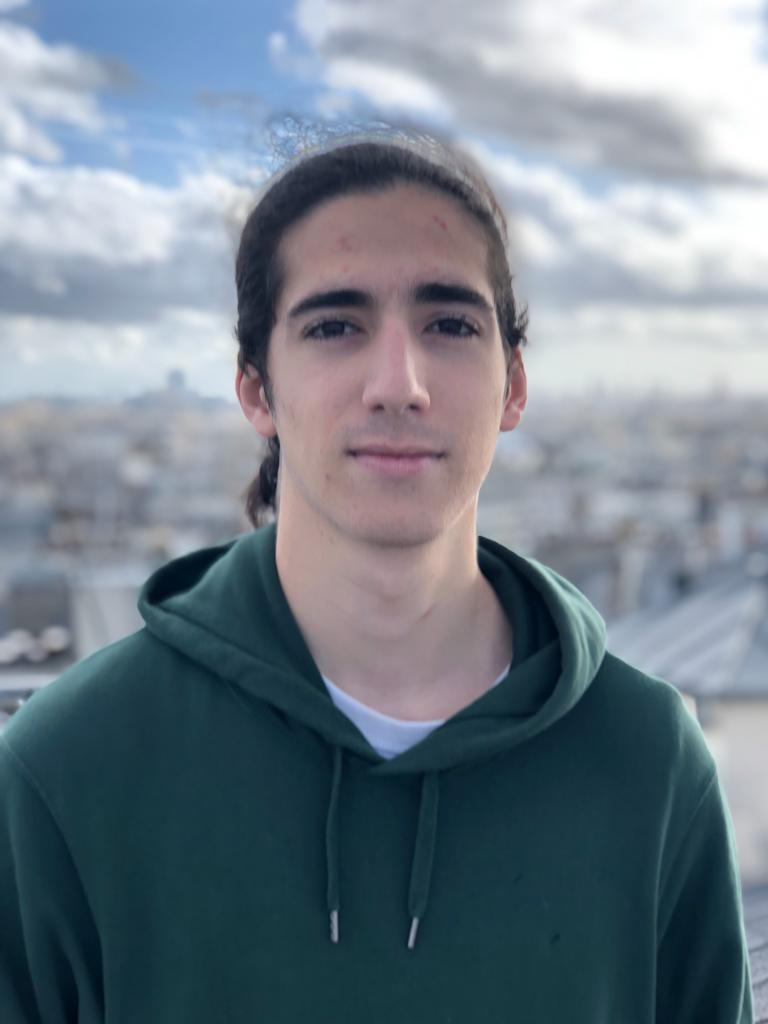
\includegraphics[width=5cm]{ulysse-mercadal.jpg}
        };
    }]
        at ([xshift=0.16666\paperwidth, yshift=-0.16666\paperwidth]current page.north west)
        {};

    % Main Content (Name, Bio, Contact) - Centered in the right 2/3 of the top bar
    \node[anchor=north, text width=0.6\paperwidth, align=center, inner sep=0pt]
        at ([xshift=0.65\paperwidth, yshift=-0.05\paperwidth]current page.north west)
    {
        \color{white} \sffamily
        {\fontsize{38}{43}\selectfont \rmfamily \textbf{Ulysse \ \ \ \ \  Mercadal}}\\[0.4cm]
        \hrule width \hsize height 1pt \vspace{0.4cm}
        {\large \href{mailto:ulyssemercadal@kakao.com}{ulyssemercadal@kakao.com} \hspace{1em} $\cdot$ \hspace{1em} \href{tel:+33620376648}{+33 6 20 37 66 48}}\\[0.4cm]
        \hrule width \hsize height 1pt \vspace{0.4cm}
        {\Large \textbf{Développeur} \hspace{1em} -- \hspace{1em} \textbf{Étudiant en 3ème année à Epitech Lyon}}\\[0.25cm]
        {\large Recherche un stage de 4 à 5 mois à partir d'avril 2026.\\
         Passionné par les architectures techniques et le travail en équipe.}
    };

    % Sidebar Content (Skills, Gap Year, Soft Skills, Languages)
    \node[anchor=north, text width=0.28\paperwidth, align=center]
        at ([xshift=0.16666\paperwidth, yshift=-0.34\paperwidth]current page.north west)
    {
        \color{white} \sffamily

        % Technical Skills
        {\Large \textbf{COMPÉTENCES TECHNIQUES}}\\[0.25cm]
        \hrule width \linewidth height 1pt \vspace{8pt}

        \raggedright
        \linespread{1.25}\selectfont

        % Low Level
        \skillRow{\iconTerminal}{\chip{C/C++} \chip{Zig} \chip{Go} \chip{Java} \chip{Python}}

        % Web App
        \skillRow{\iconWeb}{\chip{TypeScript} \chip{React} \chip{Next.js} \chip{Node.js}}

        % Mobile
        \skillRow{\iconMobile}{\chip{React Native} \chip{Flutter}}

        % CI/CD
        \skillRow{\iconLoop}{\chip{Docker} \chip{Jenkins} \chip{GitHub Actions}}

        % DB
        \skillRow{\iconDB}{\chip{PostgreSQL} \chip{MongoDB} \chip{Redis}}

        % 3D Graphics
        \iconCube \hfill \begin{minipage}[t]{0.2\paperwidth}\raggedleft \chip{OpenGL} \chip{Vulkan}\end{minipage}

        \vspace{0.7cm}
        \centering

        % Gap Year
        {\Large \textbf{ANNÉE DE CÉSURE}}\\[0.25cm]
        \hrule width \linewidth height 1pt \vspace{0.25cm}
        \textbf{En cours}\\[0.15cm]
        \chip{ICLP $|$ National Taiwan University}\\[0.15cm]
        {\small Programme intensif de chinois mandarin (Taipei)}

        \vspace{0.7cm}

        % Soft Skills
        {\Large \textbf{SOFT SKILLS}}\\[0.25cm]
        \hrule width \linewidth height 1pt \vspace{0.25cm}
        \centering
        \chip{Autonomie} \chip{Adaptabilité} \chip{Résolution de problèmes} \chip{Pédagogie} \chip{Méthodes Agiles}

        \vspace{0.7cm}

        % Languages
        {\Large \textbf{LANGUES}}\\[0.25cm]
        \hrule width \linewidth height 1pt \vspace{0.25cm}
        Français: \chip{Natif}\\[0.18cm]
        Anglais: \chip{Courant}\\[0.18cm]
        Espagnol: \chip{Avancé}\\[0.18cm]
        Chinois: \chip{En apprentissage / ICLP}
    };

    % Central White Area Content (Work Experience, Projects, Hobbies)
    \node[anchor=north west, text width=0.58\paperwidth, align=justify]
        at ([xshift=0.36\paperwidth, yshift=-0.345\paperwidth]current page.north west)
    {
        \color{discordblack} \sffamily

        % Work Experience
        {\Large \textbf{EXPÉRIENCES PROFESSIONNELLES}}\\[0.1cm]
        \hrule width \linewidth height 1pt \vspace{0.25cm}

        \blackchip{Stagiaire Développeur Full Stack} \hfill \textit{5 mois, 2025}\\[0.12cm]
        \href{https://ezyperf.com/}{\textit{Ezyperf}} \hfill \textit{Full Remote, France / Japon}\\[0.1cm]
        Développement des modules RH et du suivi des temps pour un ERP destiné aux PME et ETI en Go, TypeScript, React et Node.js en télétravail complet.
        \dottedSep

        \blackchip{Assistant Pédagogique Régional (AER)} \hfill \textit{6 mois, 2024--2025}\\[0.12cm]
        \href{https://www.ionis-group.com/}{\textit{Groupe IONIS}} \hfill \textit{Lyon, France}\\[0.1cm]
        Accompagnement et mentorat des étudiants à Epitech Lyon. Enseignement des bonnes pratiques de code, revues techniques et évaluations de projets.
        \dottedSep

        \blackchip{Stagiaire Informatique (FabLab)} \hfill \textit{5 mois, 2024}\\[0.12cm]
        \href{https://www.bpce-it.fr/}{\textit{BPCE-IT (Banque Populaire Caisse d'Epargne)}} \hfill \textit{Paris, France}\\[0.1cm]
        Expérimentation de technologies émergentes pour le 2ème groupe bancaire français. Réalisation de POCs et MVPs (LLMs, RAG, OpenTelemetry, NoSQL).

        \vspace{0.35cm}

        % Projects
        {\Large \textbf{PROJETS}}\\[0.1cm]
        \hrule width \linewidth height 1pt \vspace{0.25cm}

        \blackchiphref{https://github.com/trippier-app}{TRIPPIER} \hfill \textit{Go, Python, Next.js, Docker, Traefik}\\[0.12cm]
        Écosystème public de voyage en microservices : moteur d'indexation POI en Go, générateur d'itinéraires en Python et interface web en Next.js derrière Traefik.
        \dottedSep

        \blackchiphref{https://github.com/nicolasnny/R-TYPE}{R-TYPE} \hfill \textit{C++, OpenGL, Protocole Réseau, Asio, ECS}\\[0.12cm]
        Shoot'em up spatial 3D multijoueur en réseau avec protocole UDP/TCP binaire sur-mesure, client graphique et moteur ECS complet.
        \dottedSep

        \blackchiphref{https://github.com/ulysse-mercadal/area}{AREA} \hfill \textit{React, NestJS, Flutter, PostgreSQL, OAuth}\\[0.12cm]
        Plateforme d'automatisation de flux web et mobile (Zapier/n8n) avec éditeur de graphe de nœuds et intégrations OAuth2 multi-services.

        \vspace{0.35cm}

        % Hobbies
        {\Large \textbf{CENTRES D'INTÉRÊT}}\\[0.1cm]
        \hrule width \linewidth height 1pt \vspace{0.25cm}
        \textbf{Voyages \& Cultures :} Voyages solo en Asie de l'Est (Japon, Chine, Taïwan, Hong Kong)\\[0.15cm]
        \textbf{Montagne \& Plein air :} Randonnée, escalade, trail, sports d'hiver\\[0.15cm]
        \textbf{Technologie :} Programmation système, électronique, conception matérielle
    };
\end{tikzpicture}
\end{document}
